\documentclass[11pt,a4paper,twoside]{report}
\usepackage[utf8]{inputenc}
\usepackage[portuguese]{babel}
\usepackage[T1]{fontenc}
\setlength{\parskip}{0.15cm}
\usepackage{fancyhdr}
\usepackage{amsmath}
\usepackage{amsfonts}
\usepackage{amssymb}
\usepackage{makeidx}
\usepackage{graphicx}
\usepackage{lmodern}
\usepackage{wrapfig}
\usepackage{color}
\usepackage{float}
%\usepackage{fourier}
\usepackage[left=2cm,right=2cm,top=2cm,bottom=2cm]{geometry}
\author{Bartolomeu J. Ubisse}
\pagestyle{fancy}
\renewcommand{\headrulewidth}{0pt}
\renewcommand{\footrulewidth}{1pt}
\fancyfoot[L]{ | UEM - 2017}
\fancyfoot[c]{}
\fancyfoot[r]{\thepage}
\begin{document}


\begin{figure}[htb]

\centering

\includegraphics[scale=1]{UEM-logotipo}
\end{figure}
\centering
{ \Large Universidade Eduardo Mondlane}\\[0.3cm] 
\large Faculdade de Ci\^encias\\[0.2cm]
 \large Departamento de F\'isica\\[0.5cm]

%\textsc{Electr\^onica B\'asica} \\[1cm]
\begin{flushleft}
\tt Exame Normal - E. Anal\'ogica\hspace{0.25cm} |Data:$14/06/2017$\hspace{0.25cm}|Hora:$10:00-12:00$ hrs.\\
\hrulefill
\end{flushleft}

\begin{enumerate}
\item Explique o que entende por dopagem e qual \'e a sua finalidade.[\textit{{3.0 Valores}}]
\item Num material semicondutor cujos \'atomos tem $"j"$ electr\~oes na \'ultima camada \'e adicionado \'atomos com $"j-1"$ electr\~oes de val\^encia. Indique os portadores minorit\'arios nesse material e justifique a raz\~ao da sua escolha.[\textit{{3.0 Valores}}] 
\item Indique de uma forma sequenciada as etapas de um processo de retifica\c c\~ao e esboce a forma do sinal na saida de cada etapa.[\textit{{3.0 Valores}}]  
\item Para o circu\'ito da fig.\ref{f1}, determine as tensões de entrada  de modo que o díodo Zener funcione correctamente regulando a tens\~ao. i)- Esboce a forma do sinal de entrada  em fun\c c\~ao do tempo e indique o ripple correspondente.[\textit{{5.0 Valores}}]
\item Detemine o ganho de tens\~ao do amplificador da fig.\ref{f2} considerando que $V_T=26$mV.[\textit{{6.0 Valores}}]
\end{enumerate}
 \noindent
\begin{minipage}[c]{4cm}
 \begin{figure}[H]
\centering
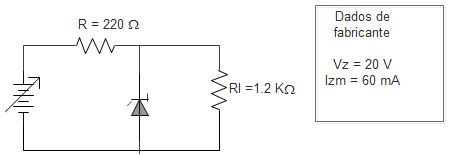
\includegraphics[scale=0.8]{cZener}
\caption{}
\label{f1}
\end{figure}
\end{minipage}\hfill
\begin{minipage}[c]{7cm}
\begin{figure}[H]
\centering
\includegraphics[scale=0.87]{test2tbj}
\caption{}
\label{f2}
\end{figure}
\end{minipage}

\vspace{0.5cm}

\Huge{Bom Trabalho !}

\newpage
\normalsize
Corre\c c\~ao\\
\hrulefill

\begin{enumerate}
\item Dopagem \'e o processo de introdu\c c\~ao de impurezas num semicondutor intr\'inseco com vista a melhorar de uma forma controlada a sua condutibilidade el\'ectrica.
\item Os portadores minorit\'arios s\~ao os electr\~oes. Considerando $"j=4"$ que \'e o caso de Sil\'icio, os \'atomos com $"j-1"$ s\~ao os do $3^{o}$grupo como \'e o caso de Boro, assim, quando os \'atomos de Borro s\~ao introduzidos num cristal intr\'inseco de Sil\'icio, tr\^es electr\~oes de Borro emparelham-se com tr\^es de Sil\'icio e fica com d\'efice de um para completar a liga\c c\~ao. Em sequ\^encia disso, o S\'ilicio cede um electr\~ao ao Borro e por essa raz\~ao fica com d\'efice de um electr\~ao e torna-se um i\~ao positivo.
\item Etapas de retifica\c c\~ao: (\textit{aceita-se tamb\'em quem usou meia onda})

\begin{figure}[H]
\centering
\includegraphics[scale=0.6]{blocosretif}
\caption{}
\end{figure}

\item Tens\~oes m\'axima e m\'inima: 

$V_{min}=\frac{R_L+R}{R_L}\times V_L \longrightarrow V_{min}=\frac{1200+220}{1200}\times 20=23.67 $V\\
\vspace{0.3cm}
$I_L=\frac{V_L}{R_L}\longrightarrow I_L=\frac{20V}{1200\Omega}=16.67mA$\\
\vspace{0.3cm}
$I_{RM}=I_{ZM}+I_L \longrightarrow I_{RM}=60 mA+16.67mA=76.67mA$\\
\vspace{0.3cm}
$V_{max}=I_{ZM}\times V_Z=36.87V$\\

\begin{enumerate}
\item[a)]

O esbo\c co \'e: 
\begin{figure}[H]
\centering
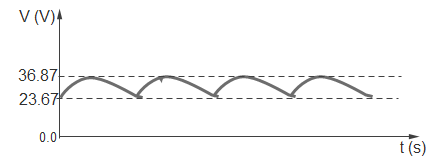
\includegraphics[scale=1]{ripple}
\caption{}
\label{f1}
\end{figure}
\end{enumerate}

\vspace{2cm}
\item Determina\c c\~ao de ganho de tens\~ao\\
\noindent
i) An\'alise cc\\
\begin{minipage}[c]{1cm}
\begin{figure}[H]
\centering
\includegraphics[scale=0.6]{analisecc}
\caption{}
\label{f4}
\end{figure}
\end{minipage}\hfill
\begin{minipage}[c]{12cm}
{$R_{BB}=\frac{R_1\times R_2}{R_1+R_2}\Longrightarrow R_{BB}=\frac{39000\times 3900}{39000+3900}=3545.45\Omega$\\

$V_{BB}=\frac{R_2}{R_1+R_2}\times V_{CC}\Longrightarrow V_{BB}=\frac{3900}{39000+3900}\times 19 = 1.73 V$\\

$R=R_3+R_4=330+1100=1430\Omega$\\

$I_C=\beta I_B$\\
$I_B+I_C=I_E \Longrightarrow I_E=(\beta +1)I_B$\\

$V_{BB}=I_BR_{BB}+V_{BE}+I_ER_E\Longrightarrow V_{BB}=I_B\left( R_{BB}+(1+\beta)R\right)+ V_{BE}$\\

Assim: $I_B=\frac{V_{BB}-V_{BE}}{R_{BB}+(1+\beta)R}\Longrightarrow I_B=\frac{1.73-0.7}{3545.45+(1+100)1430}=6.94\mu A$\\

$I_C=\beta I_B\Longrightarrow I_C=100\times 6.94\mu A =0.69 mA$\\

$I_E=(\beta +1)I_B \Longrightarrow I_E=(100 +1)\times6.94\mu A= 0.70mA$
}
\end{minipage}

\hrulefill

ii) An\'alise ac

\noindent
\begin{minipage}[c]{5cm}
\begin{figure}[H]
\centering
\includegraphics[scale=0.65]{analiseac}
\caption{}
\label{f4}
\end{figure}
\end{minipage}\hfill
\begin{minipage}[c]{8cm}
{$r_{\pi}=\frac{V_T}{I_B}\Longrightarrow r_{\pi}=\frac{26mV}{6.94\mu A}=3745.22\Omega
 $\\

$i_b=\frac{v_i}{r_{\pi}+(1+\beta)R_3}$\\

$i_c=\beta \times i_b\Longrightarrow i_c=\frac{\beta v_i}{r_{\pi}+(1+\beta)R_3}$\\

$v_o=i_c\times R_C\Longrightarrow v_o=\frac{\beta R_C }{r_{\pi}+(1+\beta)R_3}\times v_i$\\

$A_v=\frac{v_o}{v_i}\Longrightarrow A_v=\frac{\beta R_C }{r_{\pi}+(1+\beta)R_3}$\\

$ A_v=\frac{100\times4700\Omega}{3745.22\Omega+(1+100)\times 330\Omega}=12.67$\\
}
\end{minipage}
\end{enumerate}
\vspace{2cm}
\Huge{Fim !}\\
\vspace{4cm}
\normalsize
\tt Todos os coment\'arios podem ser enviados para:\\
\color{blue}bartolomeujoaquim.ubisse@gmail.com
\end{document}